\begin{frame}{Cele pracy}

    \begin{alertblock}{}
        Celem projektu przedstawionego w niniejszej pracy było opracowanie i weryfikacja koncepcji przedwzmacniacza dedykowanego do wielokanałowej sondy neuronalnej umożliwiającej rejestrację aktywności neuronalnej mózgu.
    \end{alertblock}

    \begin{block}{Główne zadania}
        \begin{itemize}
            \item Kompleksowa analiza zniekształceń nieliniowych we wzmacniaczach neuronalnych
            \item Optymalizacja kluczowych parametrów przedwzmacniaczy neuronalnych
            \item  Projekt układu scalonego, obwodu drukowanego oraz systemu akwizycji danych
            \item Wykonanie testów elektronicznych oraz analiza parametrów i charakterystyk opracowanego układu scalonego
            \item Weryfikacja funkcjonalności opracowanego przedwzmacniacza  w eksperymentach neurobiologicznych i analiza zebranych danych
        \end{itemize}
    \end{block}

    
\end{frame}

\begin{frame}{Zakresy amplitud i częstotliwości sygnałów neuronowych w różnych technikach rejestracji}
    \begin{columns}
        \column{.48\textwidth}
        \vspace{-2em}

        \begin{figure}[H]
            \includegraphics[scale=0.2]{ch1/brain.jpg}
          \end{figure}
          \begin{block}{Metody rejestracji}
            \begin{itemize}
                {\renewcommand\normalsize{\small}%
                \normalsize
                \item LFP -- Local Field Potential
                \item AP --  Action Potential
                \item ECoG -- Electrocorticography
                \item EEG -- Electroencephalography
                }
            \end{itemize}
        \end{block}
        \column{.48\textwidth}
        \vspace{-2em}

        \begin{figure}[H]
            \centering
            \includegraphics[scale=1.0]{ch1/lfp_ap_spectrum}  
            \end{figure}	
    \end{columns}
    
\end{frame}

\begin{frame}{Kierunki rozwoju współczesnych systemów pomiarowych i matryc mikroelektrodowych}
   
    \begin{columns}
    \column{.55\textwidth}

    \begin{block}{Techniki pomiarowe wewnątrz i \\
        zewnątrzkomórkowe w neurobiologii}
        \begin{itemize}
            \item różne amplitudy sygnałów
            \item inwazyjność badań
            \item obszar badań 
        \end{itemize}
    \end{block}
    \column{.4\textwidth}
    \vspace{-3em} %5mm vertical space

        \begin{columns}
        \column{.5\textwidth}
        \begin{figure}[H]
            \includegraphics[scale=0.13]{ch2/masm64Dsharp.png}
        \end{figure}

        \column{.5\textwidth}
            \begin{figure}[H]
                \includegraphics[scale=0.13]{ch2/utahArr.png}
            \end{figure}
        \end{columns}
    \end{columns}

    \begin{columns}

        \column{.55\textwidth}
        % \vspace{-3em} %5mm vertical space

        \begin{figure}[H]
            \includegraphics[scale=0.45]{ch1/intra-extra.png}  
        \end{figure}

        \column{.4\textwidth}
        \vspace{-2em} %5mm vertical space
        \begin{figure}[H]
                % \includegraphics[scale=0.25]{ch1/ap.png}
            \includegraphics[scale=0.25]{ch2/neuropixel10.png}  
        \end{figure}


    \end{columns}


    
\end{frame}

% \begin{frame}{Kierunki rozwoju współczesnych systemów pomiarowych i matryc mikroelektrodowych}
%     \vspace{-5mm} %5mm vertical space

%     \begin{columns}[t]
%         \column{.3\textwidth}
%         \begin{figure}[H]
%             \includegraphics[scale=0.35]{ch2/neuropixel10.png}  
%         \end{figure}

%         \column{.3\textwidth}
%         \begin{figure}[H]
%             \includegraphics[scale=0.35]{ch2/argo.jpeg}  
%         \end{figure}

%         \column{.35\textwidth}
%         \begin{figure}[H]
%             \includegraphics[scale=0.2]{ch2/masm64Dsharp.png}
%         \end{figure}

%         \begin{figure}[H]
%             \includegraphics[scale=0.25]{ch2/utahArr.png}
%         \end{figure}

%     \end{columns}


% \end{frame}





\begin{frame}{Kanał rejestracji neuronowej z wykorzystaniem mikroelektrod zewnątrzkomórkowych}
\vspace{-1em}
    \begin{columns}
        \column{.48\textwidth}
        \begin{figure}[H]
            \centering
            \includegraphics[scale=0.25]{ch2/chemNeuroInterface.png} 

        \end{figure}
        \begin{figure}[H]
            \centering
            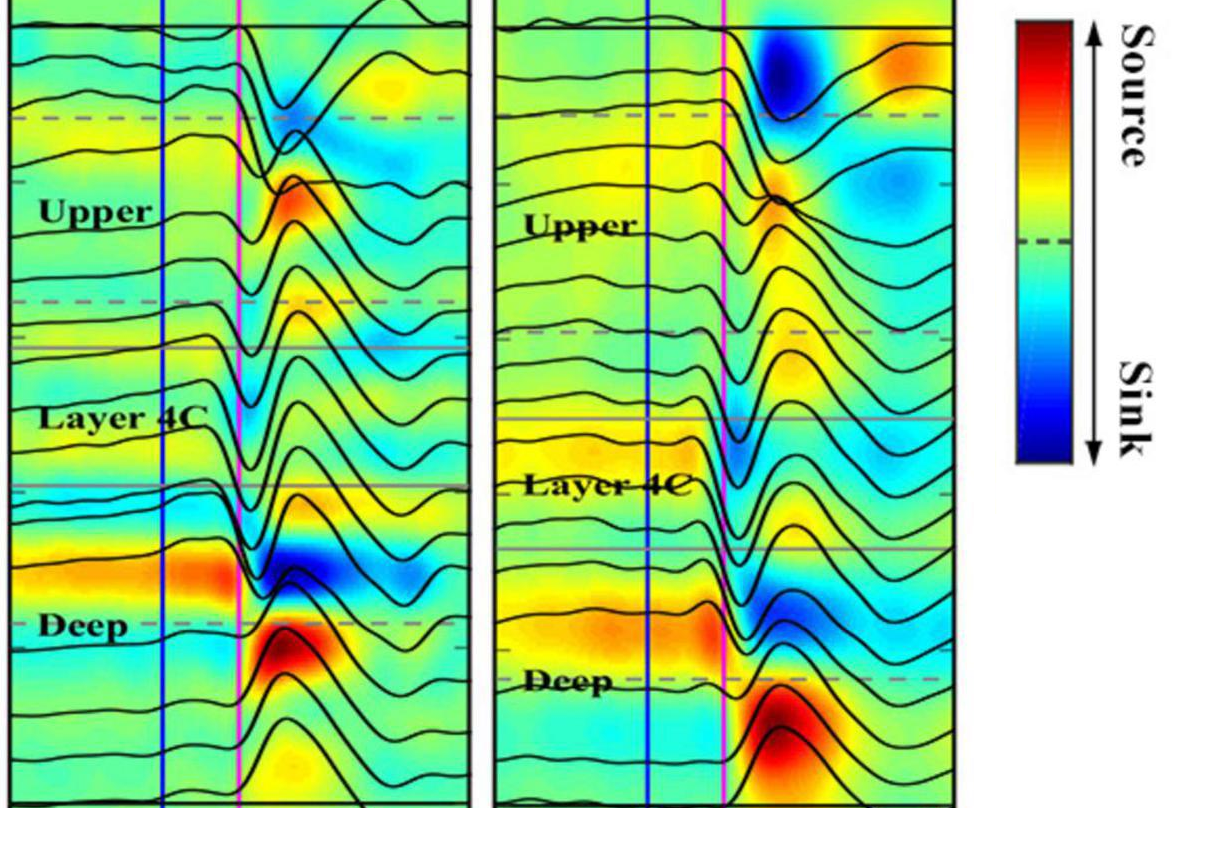
\includegraphics[scale=0.25]{ch1/lfp.png} 

          \end{figure}

        \column{.48\textwidth}
        \begin{block}{Wymagania stawiane interfejsom neuroelektronicznym umożliwiającym rejestrację sygnałów LFP i AP}
            \begin{itemize}
                \item Stałe napięcie na styku elektrody -- do $\SIrange{1}{2}{\volt}$ 
                \item Szumy $<\SI{10}{\micro\volt}$ dla pasma LFP i AP
                \item Liniowość rejestrowanego sygnału
                \item Pobór mocy -- limit ogrzewania tkanki mózgowej --  mniej niż  $\SI{1}{\degreeCelsius}$ 
                \item Zróżnicowane sygnały: amplituda do $\SI{10}{\milli\volt_{pp}}$ dla LFP i od  $\SI{50}{\micro\volt}$ dla AP
                \item Skalowalność -- tysiące kanałów dla przyszłych systemów
            \end{itemize}
        \end{block}
        % Schemat typowego kanału rejestracji neuronowej i modelu elektrycznego interfejsu tkanka-mikroelektroda: 
        % $Z_{CPA}$ -- element o stałej fazie, 
        % $R_{CT}$ -- rezystancja dla przepływającego prądu przez elektrodę,  
        % $R_{SP}$ -- rezystancja rozproszona elektrolitu, 
        % $V_{HC}$ -- potencjał w interfejsie elektroda -- tkanka. 
 
    \end{columns}
\end{frame}


% \begin{frame}{Sprzężenie zmiennoprądowe}
%     \begin{columns}
%         \column{.48\textwidth}

%     \begin{figure}[H]
%         \centering
%         \includegraphics[scale=0.75]{ch2/conceptAC_Harrison.pdf} 
%     \end{figure}
%     \column{.48\textwidth}
%     \begin{alertblock}{Wyzwania zwiazane z sprzęzeniem AC}
%         \begin{itemize}
%             \item Niska dolna częstotliwość graniczna rzędu~$\SI{\sim 1}{\hertz}$ 
%             \item Pojemności w technologi CMOS są rzędu $\SI{}{\femto\farad\per\micro\metre\squared}$
%             \item Rezystancja sprzężenia zwrotnego w zakresie $\SI{}{\tera\ohm}$
%         \end{itemize}
%     \end{alertblock}
%     \begin{exampleblock}{Zalety}
%         \begin{itemize}
%             \item Usunięcie składowej stałej od elektrody niezależnie od jej wartości
%             \item Wydajność szumowa i poboru mocy
%         \end{itemize}
%     \end{exampleblock}
% \end{columns}

% \end{frame}



% \begin{frame}{Sprzężenie stałoprądowe}
%     \begin{columns}
%         \column{.48\textwidth}
%         \begin{figure}[H]
%             \centering
%             \includegraphics[scale = 0.5]{ch2/dc_coupling.pdf}
%         \end{figure}

%     \column{.48\textwidth}
%     \begin{alertblock}{Wyzwania zwiazane z sprzęzeniem DC}
%         \begin{itemize}
%             \item Duża wrażliwość na offset
%             \item Pobór mocy
%         \end{itemize}
%     \end{alertblock}
%     \begin{exampleblock}{Zalety}
%         \begin{itemize}
%             \item Brak konieczności używania dużych rezystancji w pętli sprzężenia zwrotnego
%         \end{itemize}

%         \begin{figure}[H]
%             \centering
%             \includegraphics[scale=0.5]{ch2/dc-integrator.pdf} 
%         \end{figure}

%     \end{exampleblock}
% \end{columns}

% \end{frame}

\begin{frame}{Sprzężenie zmiennoprądowe i stałoprądowe}
    

    \begin{columns}
        \column{.55\textwidth}
        \vspace{-1em} %5mm vertical space

        \begin{figure}[H]
            \centering
            \includegraphics[scale=0.5]{ch2/conceptAC_Harrison.pdf} 
        \end{figure}
        \vspace{-2em} %5mm vertical space

        {\renewcommand\normalsize{\small}%
        \normalsize
    
        % \begin{alertblock}{Wyzwania zwiazane z sprzęzeniem AC}
    %5mm vertical space
    
        % \begin{exampleblock}{Zalety}
        % \begin{exampleblock}{Sprzężenie zmiennoprądowe}
        \begin{exampleblock}{}

            \begin{itemize}
                \item Całkowite usunięcie napięcia stałego na elektrodzie 
                \item Konieczność implementacji filtru górnoprzepustowego z dolną częstotliwością graniczną rzędu~$\SI{\sim 1}{\hertz}$ 
                \item Ograniczenia na pojemności kondensatorów w technologii CMOS $\sim\SI{}{\pico\farad}$
                \item  Wymagane rezystancje  $\sim\SI{}{\tera\ohm}$
            \end{itemize}
        \end{exampleblock}
    
        }


        \column{.43\textwidth}
        \vspace{-3em} %5mm vertical space

        \begin{figure}[H]
            \hspace{-2em} %5mm vertical space
            \includegraphics[scale = 0.48]{ch2/dc_coupling.pdf}
        \end{figure}


    {\renewcommand\normalsize{\small}%
    \normalsize
    % \begin{alertblock}{Wyzwania zwiazane z sprzęzeniem DC}
    \vspace{-1em} %5mm vertical space

    % \begin{alertblock}{Sprzężenie stałoprądowe}
        \begin{alertblock}{}

        \begin{itemize}
            \item Alternatywne podejście do eliminacji składowej stałej napięcia na styku elektrody i tkanki
        \end{itemize}
    \end{alertblock}
    }

    \end{columns}

\end{frame}
